% !TeX root = ../collection-solutions.tex

% Comparisons 3
\titledquestion{Social comparisons} Consider the model of social comparisons by \citet{drechsel2025falling-behind} 
    with three types ($P$, $M$, $R$), weights $\vec \omega = (\omega_P, \omega_M, \omega_R)$ 
    and the following comparison network $G$.

    \begin{center}
        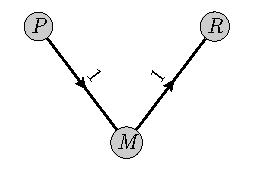
\includegraphics{comparisons/comparison-network-richer}
    \end{center}

    \begin{parts}
        \part Let $\tilde \phi = \kappa_1 \phi$. Compute the social externality matrix $L$.

        \begin{solution}
        
            $G = \begin{pmatrix}
                0 & 1 & 0 \\ 0 & 0 & 1 \\ 0 & 0 & 0
            \end{pmatrix}$, 
            %
            $G^2 = \begin{pmatrix}
                0 & 0 & 1 \\ 0 & 0 & 0 \\ 0 & 0 & 0
            \end{pmatrix}$,
            %
            $G^3 = G^4 = \cdots = 0 \in \mathbb{R}^{3 \times 3}$

            Hence,

            $L = \sum_{i=1}^\infty \phi^i G^i = \begin{pmatrix}
                0 & \tilde \phi & \tilde \phi^2 \\
                 0 & 0 & \tilde \phi \\ 
                 0 & 0 & 0 \\
            \end{pmatrix}$
        \end{solution}

        \uplevel{Consider a \emph{low inequality} steady state 
        with incomes $\underline{\vec y} = (\underline y^P, \underline y^M, \underline y^R)$
        and a \emph{high inequality} steady state 
        with incomes $\overline{\vec y} = (\overline y^P, \overline y^M, \overline y^R)$.
        
        In the \emph{high inequality} steady state $R$ is richer, and $P$ is poorer than in the \emph{low inequality} state:%
        %
        \begin{equation*}
            \omega_R \Delta y^R = - \omega_P \Delta y^P > 0, \quad \text{and } \Delta y^M = 0.
        \end{equation*}
        where $\Delta y^i = \overline y^i - \underline y^i$.
        }
        \part Will aggregate debt $D$ be higher or lower in the high inequality steady state? \emph{Use the relevant result from Drechsel-Grau and Greimel (2024).}

        \begin{solution}
            The relevant condition is  $$D(\overline{ \vec y}) > D(\underline{\vec y}) \iff \frac{b_P}{\omega_P} < \frac{b_R}{\omega_R}.$$

            Note that $b_P = 0$ and $b_R = \omega_M \tilde \phi + \omega_P \tilde \phi^2 > 0$. Hence the above condition is satisfied (higher debt in \emph{high inequality} steady state).
        \end{solution}
       
        \part Interpret this result and discuss its relevance.

        \begin{solution}
            \begin{itemize}
                \item Income inequality has been rising in the past decades: The income share of the bottom 50\% has fallen, while the income share of the top 10\% has increased. So we can interpret the two steady states corresponding to some decades age (e.g.\ 1980) vs now.

                \item Empirically, social comparisons tend to be upward looking, so the given $G$ might be a good approximation of reality.
    
                \item This model predicts that increasing inequality \emph{causes} a rise in household debt.
                
                \item Consistent with this, the data show that there is a positive \emph{correlation} between debt and inequality.
            \end{itemize}
        \end{solution}
    \end{parts}